
\documentclass{beamer}

\usepackage{cmap}                                       % поиск в PDF
\usepackage[T2A]{fontenc}                       % кодировка
\usepackage[utf8]{inputenc}                     % кодировка исходного текста
\usepackage[english,russian]{babel}     % локализация и переносы

\usepackage{graphicx}
\graphicspath{{images/}}

\usepackage{amsmath}

\usepackage{algorithm}
\usepackage[noend]{algpseudocode}

\algdef{SE}[DOWHILE]{Do}{doWhile}{\algorithmicdo}[1]{\algorithmicwhile\ #1}%

%% \usetheme{Berkeley}
%% \usecolortheme{beaver}
\definecolor {processblue}{cmyk}{0.96,0,0,0}

\DeclareMathOperator*{\argmax}{arg\,max}

\usepackage{tikz}
\usetikzlibrary {automata, arrows, positioning}
%% \usepackage{tikz,fullpage}

\logo{
\includegraphics[height=0.8cm]{bsu_logo_ru.eps}}
\title{Основы теории скрытых марковских моделей}
\author{Кузьмин А.А.}
\institute[]{\url{http://rfe.bsu.by/}}

\begin{document}

\begin{frame}
  \maketitle
\end{frame}

\section{Содержание}
%% Непосредственно речевого сигнала мы пока касаемся косвенно,
%% поскольку, сначала необходимо представить мат. аппарат
\begin{frame} \label{cont}
  \frametitle{\insertsection}
  \begin{enumerate}
    \item Понять проблему из-за которой представление сигнала как случайного вектора не достаточно \pause
    \item Понять что из себя представляют \alert{скрытые марковские модели (СММ)} в самом простом случае и из чего они состоят\pause
    \item Познакомиться с тем как ими правильно пользоваться \\
      \pause \alert{$3$ базовые проблемы СММ}
  \end{enumerate}
\end{frame}

\section{Пролема с представлением сигнала как случайного вектора}
\begin{frame}
  \frametitle{\insertsection}
  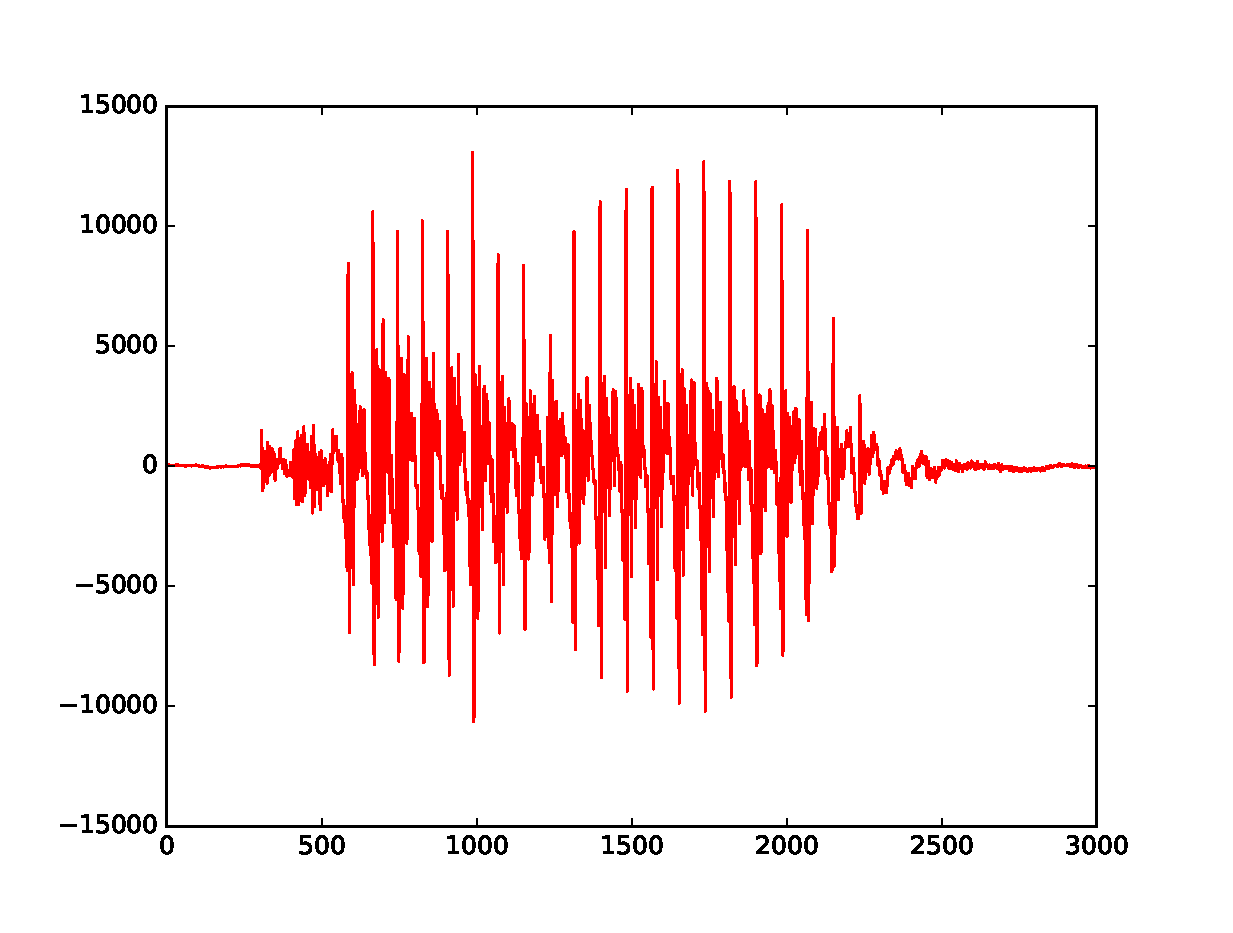
\includegraphics[width=0.8\textwidth]{a_short.eps}
\end{frame}

\section{Пролема с представлением сигнала как случайного вектора}
\begin{frame}
  \frametitle{\insertsection}
  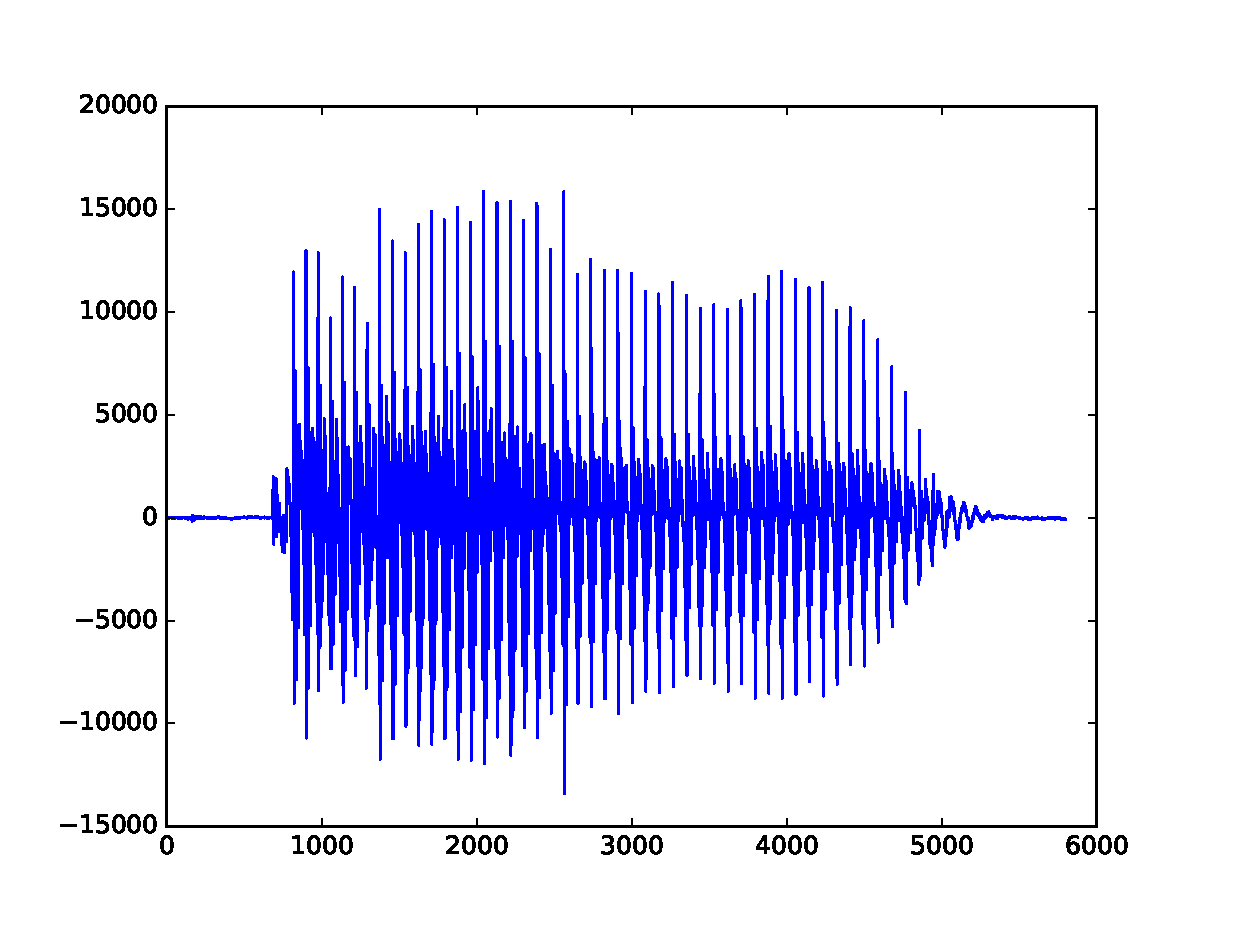
\includegraphics[width=0.8\textwidth]{a_long.eps}
\end{frame}

\section{Пролема с представлением сигнала как случайного вектора}
\begin{frame}
  \frametitle{\insertsection}
  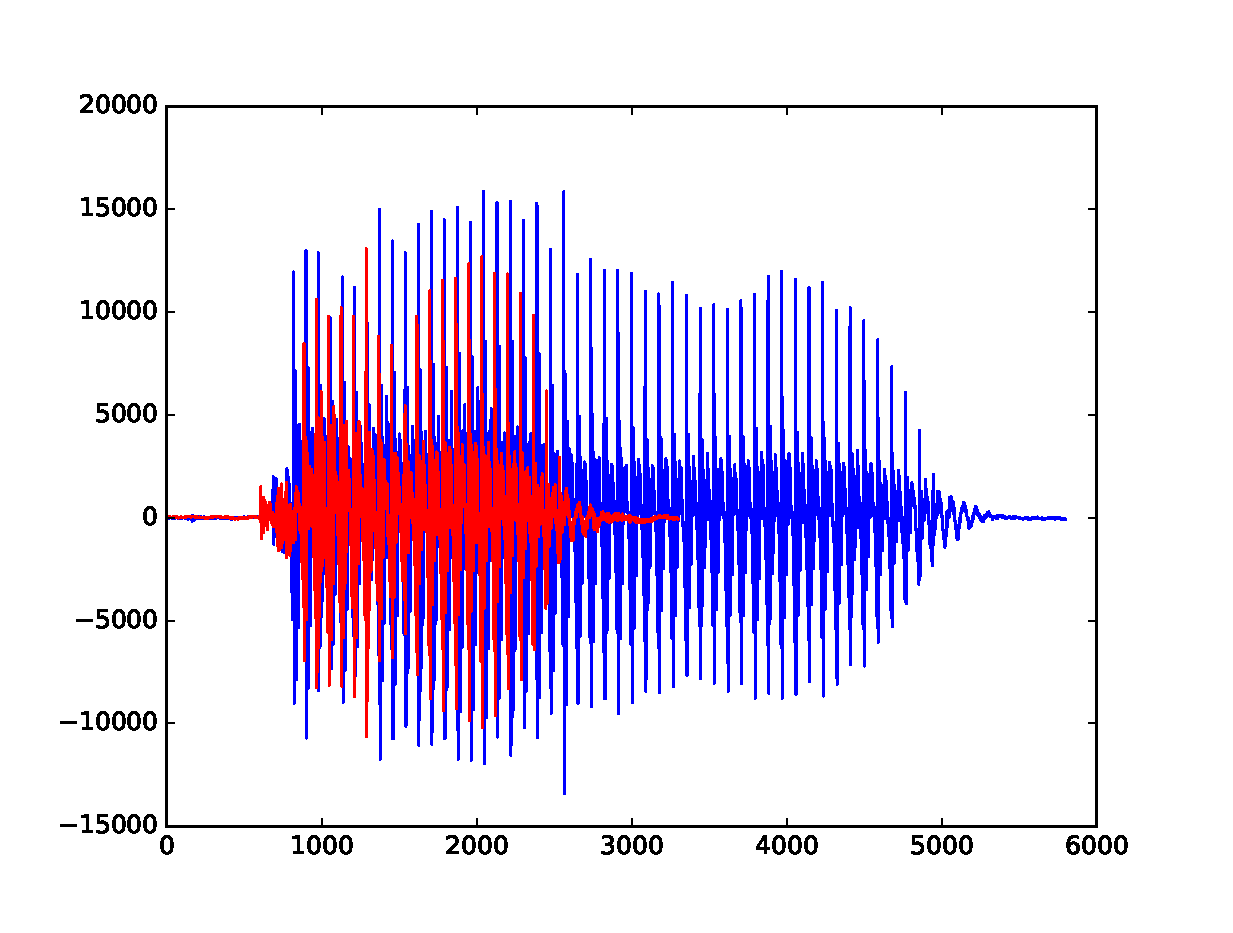
\includegraphics[width=0.8\textwidth]{a_long_short.eps}
\end{frame}

\section{Марковский процесс дискретный по времени}
\subsection{Основные понятия}

%% Будем стараться быть проблема-ориентированными
\begin{frame}
  \frametitle{\insertsection}
  \framesubtitle{Система включающая $N$ состояний $S_1, S_2, \ldots, S_N$}
  %% 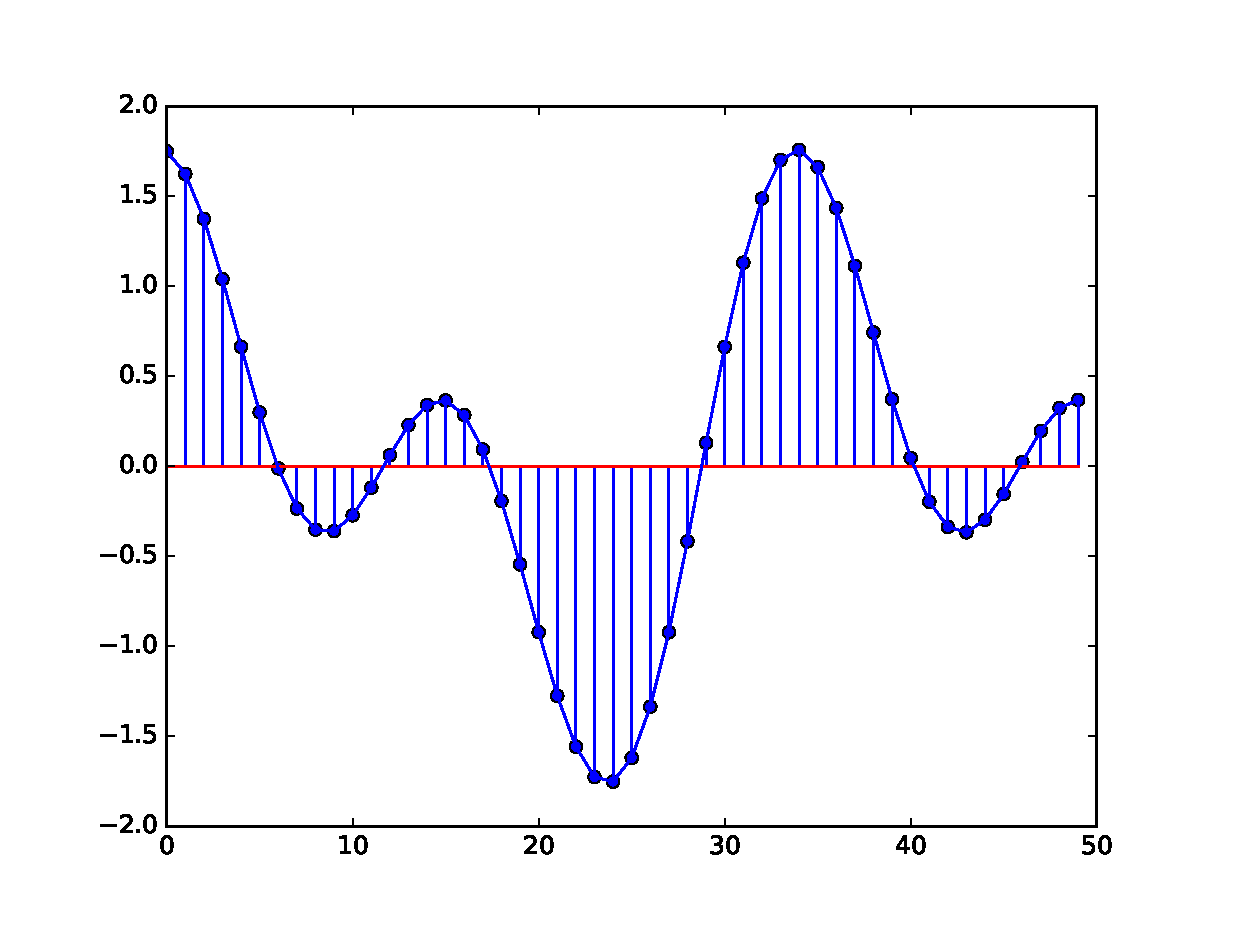
\includegraphics[width=0.8\textwidth]{tovec.eps}

  \begin{figure}
    \centering
    \begin{tikzpicture}[->, >=stealth', auto, node distance =3 cm and 4cm, on grid, semithick]
      \tikzstyle{every state}=[fill=white,draw=black,thick,text=black,scale=0.8]
      \node[state] (C) {$S_3$};
      \node[state] (A) [above left = of C] {$S_1$};
      \node[state] (B) [above right = of C] {$S_2$};
      \path (A) edge [loop left] node {$a_{11}$} (A);
      \path (C) edge [bend left =25] node {$a_{31}$} (A);
      \path (A) edge [bend right = -15] node[below =0.15 cm] {$a_{13}$} (C);
      \path (A) edge [bend left =25] node[above] {$a_{12}$} (B);
      \path (B) edge [bend left =15] node[below =0.15 cm] {$a_{21}$} (A);
      \path (C) edge [bend left =15] node[below =0.15 cm] {$a_{32}$} (B);
      \path (B) edge [bend right = -25] node[below =0.15 cm] {$a_{23}$} (C);
    \end{tikzpicture}
  \end{figure}
\end{frame}

\begin{frame}
  \frametitle{\insertsection}
    \framesubtitle{\insertsubsection}
  \begin{itemize}
    \item $S_1, S_2, \ldots, S_N$
    \item $t_1, t_2, \ldots$
    \item состояние в момент времени $t$: $q_t$
    \item полное вероятностное описание: $P(q_t = S_i | q_{t - 1} = S_j, q_{t - 2} = S_k, \ldots) = $ \pause $P(q_t = S_i | q_{t - 1} = S_j)$
      \\ для цепи Маркова
      %% Вероятность находится в том или ином состоянии в данный момент
      %% с учетом того в каких состояниях находилась система до этого
  \end{itemize}
\end{frame}

\begin{frame}
  \frametitle{\insertsection}
    \framesubtitle{\insertsubsection}
  \begin{itemize}
    \item $a_{ij} = P(q_t = S_i | q_{t - 1} = S_j)$ \pause
    \item $a_{ij} \ge 0, \forall i, \forall j$ \pause
    \item $\displaystyle \sum_{j = 1}^{N} a_{ij} = 1$
  \end{itemize}
\end{frame}

\subsection{Конкретный пример}

\begin{frame}
  \frametitle{\insertsection}
    \framesubtitle{\insertsubsection}
  \begin{itemize}
    \item $S_1$: ``\textit{Снег}'' (``\textit{Дождь}'')
    \item $S_2$: ``\textit{Пасмурно}''
    \item $S_3$: ``\textit{Солнечно}''
  \end{itemize}
  \begin{equation*}
    A = \{a_{ij}\} =
    \begin{bmatrix}
      0.4 & 0.3 & 0.3 \\
      0.2 & 0.6 & 0.2 \\
      0.1 & 0.1 & 0.8 \\
    \end{bmatrix}
  \end{equation*}
\end{frame}

\begin{frame}
  \frametitle{\insertsection}
    \framesubtitle{\insertsubsection}
    \begin{figure}
    \centering
    \begin{tikzpicture}[->, >=stealth', auto, node distance =3 cm and 4cm, on grid, semithick]
      \tikzstyle{every state}=[fill=white,draw=black,thick,text=black,scale=0.8]
      \node[state] (C) {$S_3$};
      \node[state] (A) [above left = of C] {$S_1$};
      \node[state] (B) [above right = of C] {$S_2$};
      \path (A) edge [loop left] node {$0.4$} (A);
      \path (B) edge [loop right] node {$0.6$} (B);
      \path (C) edge [loop below] node {$0.8$} (C);
      \path (C) edge [bend left =25] node {$0.1$} (A);
      \path (A) edge [bend right = -15] node[below =0.15 cm] {$0.3$} (C);
      \path (A) edge [bend left =25] node[above] {$0.3$} (B);
      \path (B) edge [bend left =15] node[below =0.15 cm] {$0.2$} (A);
      \path (C) edge [bend left =15] node[below =0.15 cm] {$0.1$} (B);
      \path (B) edge [bend right = -25] node[below =0.15 cm] {$0.2$} (C);
    \end{tikzpicture}
  \end{figure}
\end{frame}

\begin{frame} \label{example_begin}
  \frametitle{\insertsection}
  \framesubtitle{\insertsubsection}
  Какова вероятность такого прогноза на неделю: \\
  ``\textit{\small{солнечно-солнечно-дождь-дождь-солнечно-пасмурно-солнечно}}''\\
  Формально: $O = S_3, S_3, S_1, S_1, S_3, S_2, S_3$ \pause

  \begin{eqnarray*}
    P(O | \text{Model}) & = & P(S_3, S_3, S_1, S_1, S_3, S_2, S_3 | \text{Model})\\
    & = & P(S_3) \cdot P(S_3|S_3) \cdot P(S_1|S_3) \cdot P(S_1|S_1) \cdot \\
    && P(S_3|S_1) \cdot P(S_2|S_3) \cdot P(S_3|P_2) \\
    & = & \pi_3 \cdot a_{33} \cdot a_{13} \cdot a_{11} \cdot a_{31}\cdot a_{23} \cdot a_{32}
  \end{eqnarray*}
  где $\pi_i = P(q_1 = S_i)$
\end{frame}

\begin{frame} \label{example_begin}
  \frametitle{\insertsection}
  \framesubtitle{\insertsubsection}
  Какова вероятность такого прогноза на неделю: \\
  ``\textit{\small{солнечно-солнечно-дождь-дождь-солнечно-пасмурно-солнечно}}''\\
  Формально: $O = S_3, S_3, S_1, S_1, S_3, S_2, S_3$

  \begin{eqnarray*}
    P(O | \text{Model}) & = & 1 \cdot (0.8)(0.1)(0.4)(0.3)(0.1)(0.2) \\
    & = & 1.920 \times 10^{-4}
  \end{eqnarray*}
\end{frame}


\section{Скрытые марковские модели}

\subsection{Предварительные примеры. Монеты}

\begin{frame}
  \frametitle{\insertsection}
  \framesubtitle{\insertsubsection}
  \begin{figure}
    \begin{center}
      \begin{tikzpicture}[->, >=stealth', auto, semithick, node distance=3cm]
        \tikzstyle{every state}=[fill=white,draw=black,thick,text=black,scale=1]
        \node[state]    (A)                     {$1$};
        \node[state]    (B)[right of=A]   {$2$};
        \path
        (A) edge[loop left]     node{$P(H)$}         (A)
        edge[bend left]     node{$1 - P(H)$}     (B)
        (B) edge[loop right]    node{$1 - P(H)$}      (B)
        edge[bend left,above]     node{$P(H)$}         (A);
      \end{tikzpicture}
    \end{center}
  \end{figure} \pause
  \begin{equation*}
    \begin{matrix}
      O & = & H & H & T & H & T & T & H & \ldots \\
      S & = & 1 & 1 & 2 & 1 & 2 & 2 & 1 & \ldots
    \end{matrix}
  \end{equation*}
\end{frame}

\begin{frame}
  \frametitle{\insertsection}
  \framesubtitle{\insertsubsection}
  \begin{figure}
    \begin{center}
      \begin{tikzpicture}[->, >=stealth', auto, semithick, node distance=3cm]
        \tikzstyle{every state}=[fill=white,draw=black,thick,text=black,scale=1]
        \node[state]    (A)                     {$1$};
        \node[state]    (B)[right of=A]   {$2$};
        \path
        (A) edge[loop left]     node{$a_{11}$}         (A)
        edge[bend left]     node{$1 - a_{11}$}     (B)
        (B) edge[loop right]    node{$a_{22}$}      (B)
        edge[bend left,above]     node{$1 - a_{22}$}         (A);
      \end{tikzpicture}
    \end{center}
  \end{figure} \pause
  \begin{equation*}
    \begin{matrix}
      P(H) = P_1     & P(H) = P_2 \\
      P(T) = 1 - P_1 & P(T) = 1 - P_2
    \end{matrix}
  \end{equation*} \pause
  \begin{equation*}
    \begin{matrix}
      O & = & H & H & T & H & T & T & H & \ldots \\
      S & = & 2 & 1 & 2 & 2 & 1 & 1 & 1 & \ldots
    \end{matrix}
  \end{equation*}
\end{frame}

\begin{frame}
  \frametitle{\insertsection}
    \framesubtitle{\insertsubsection}
    \begin{figure}
    \centering
    \begin{tikzpicture}[->, >=stealth', auto, node distance =2 cm and 3cm, on grid, semithick]
      \tikzstyle{every state}=[fill=white,draw=black,thick,text=black,scale=0.8]
      \node[state] (C) {$3$};
      \node[state] (A) [above left = of C] {$1$};
      \node[state] (B) [above right = of C] {$2$};
      \path (A) edge [loop left] node {$a_{11}$} (A);
      \path (B) edge [loop right] node {$a_{22}$} (B);
      \path (C) edge [loop below] node {$a_{33}$} (C);
      \path (C) edge [bend left =25] node {$a_{31}$} (A);
      \path (A) edge [bend right = -15] node[below =0.15 cm] {$a_{13}$} (C);
      \path (A) edge [bend left =25] node[above] {$a_{12}$} (B);
      \path (B) edge [bend left =15] node[below =0.15 cm] {$a_{21}$} (A);
      \path (C) edge [bend left =15] node[below =0.15 cm] {$a_{32}$} (B);
      \path (B) edge [bend right = -25] node[below =0.15 cm] {$a_{23}$} (C);
    \end{tikzpicture}
    \end{figure} \pause
    $P(H) = P_1 \qquad P(H) = P_2  \qquad P(H) = P_3 $ \\
    $ P(T) = 1 - P_1 \qquad P(T) = 1 - P_2 \qquad P(T) = 1 - P_3 $
    \pause

    $\displaystyle
    \begin{matrix}
      O & = & H & H & T & H & T & T & H & \ldots \\
      S & = & 3 & 1 & 2 & 3 & 1 & 1 & 2 & \ldots
    \end{matrix}
    $

\end{frame}

\subsection{Предварительные примеры. Карзины с шарами}

\begin{frame}
  \frametitle{\insertsection}
  \framesubtitle{\insertsubsection}

  \begin{table}
    \begin{tabular}{ccc}
      КАРЗИНА $1$ & КАРЗИНА $2$ & КАРЗИНА $3$ \\
      $P(\text{RED}) = b_1(1)$ & $P(\text{RED}) = b_2(1)$ & $P(\text{RED}) = b_3(1)$ \\
      $P(\text{BLUE}) = b_1(2)$ & $P(\text{BLUE}) = b_2(2)$ & $P(\text{BLUE}) = b_3(2)$ \\
      $P(\text{GREEN}) = b_1(3)$ & $P(\text{GREEN}) = b_2(3)$ & $P(\text{GREEN}) = b_3(3)$ \\
      \vdots & \vdots & \vdots \\
      $P(\text{BLACK}) = b_1(M)$ & $P(\text{BLACK}) = b_2(M)$ & $P(\text{BLACK}) = b_3(M)$ \\
    \end{tabular}
  \end{table}

  \begin{equation*}
  O = \text{GREEN},  \text{BLACK}, \text{BLUE}, \text{RED}, \text{RED}, \ldots, \text{BLUE}
  \end{equation*}

\end{frame}

\subsection{Ингредиенты}

\begin{frame}
  \frametitle{\insertsection}
  \framesubtitle{\insertsubsection}
  %% Любая теория начинается с базовых понятий (или с проблемы)
  \begin{enumerate}
  \item Количество состояний: $N$ \pause
  \item Множество наблюдаемых значений $\{v_k\}$ с количеством элементов $M$ \pause
  \item Матрица вероятностей перехода из одного состояния в другу: \\
    $A = \{a_{ij}\}$, где $a_{ij} = P(q_t = S_i | q_{t - 1} = S_j)$ \pause
  \item Вероятность получить то или иное наблюдение при условии нахождения в определенном состоянии: \\
    $B = {b_i(k)}$, где $b_i(k) = P(O_t = v_k | q_t = S_i)$, \\
    $1 \le i \le N$, $1 \le k \le M$ \pause
    \item Начальные вероятности: $\pi_i = P(q_1 = S_i)$, $1 \le i \le M$
  \end{enumerate}

  \pause
  \begin{equation*}
    \lambda = \{A, B, \pi\}  %% Остальное понятно из приложения
  \end{equation*}

\end{frame}

\section{Три базовые проблемы СММ}
%% Или как пользоваться СММ
\subsection{Проблема 1}
%% Задачка, которую надо решить поскольку очень нужен ответ

\begin{frame}
  \frametitle{\insertsection}
  \framesubtitle{\insertsubsection}
  \begin{itemize}
  \item Дана последовательность наблюдений: $O = O_1, O_2, \ldots, O_T$ \pause
  \item Есть модель $\lambda = \{A, B, \pi \}$ \pause
  \item Какова вероятность того что последовательность была сгенерирована данной моделью: \\
    $P(O | \lambda) = ?$
  \end{itemize}
\end{frame}

\subsection{Проблема 2}

\begin{frame}
  \frametitle{\insertsection}
  \framesubtitle{\insertsubsection}
  \begin{itemize}
  \item Дана последовательность наблюдений: $O = O_1, O_2, \ldots, O_T$ \pause
  \item Есть модель $\lambda = \{A, B, \pi \}$ \pause
  \item Какова последовательность состояний модели $Q = q_1, q_2, \ldots, q_T$, которая наилучшим (в некотором смысле) образом соответствует $O$?
  \end{itemize}
\end{frame}

\subsection{Проблема 3}

\begin{frame}
  \frametitle{\insertsection}
  \framesubtitle{\insertsubsection}
  \begin{itemize}
  \item Дана последовательность наблюдений: $O = O_1, O_2, \ldots, O_T$ \pause
  \item Каким образом выбрать значения параметров $\{A, B, \pi\}$ модели так что бы максимизировать значение $P(O|\lambda)$
  \end{itemize}
\end{frame}


\section{Проблема 1. Вероятность появления последовательности}
\subsection{Первая попытка}

\begin{frame}
  \frametitle{\insertsection}
  \framesubtitle{\insertsubsection}
  \begin{itemize}
  \item Для одной конкретной последовательности $Q = q_1, q_2, \ldots, q_T$: \\ $\displaystyle P(O | Q, \lambda) = \prod_{t = 1}^{T} P(O_t | q_t, \lambda)$
    \pause
  \item $\displaystyle P(O | Q, \lambda) = b_{q_1}(O_1) \cdot b_{q_2}(O_2) \ldots b_{q_T}(O_T)$ \pause
  \item $\displaystyle P(Q | \lambda) = \pi_{q_1} \cdot a_{q_1q_2} \cdot a_{q_2q_3} \ldots a_{q_{T - 1}q_T}$ \pause
  \item $\displaystyle P(O, Q | \lambda) = P(Q | \lambda) \cdot P(O | Q, \lambda)$
    \pause
  \item Суммируем по всем возможным последовательностям: $\displaystyle P(O | \lambda) = \sum_{\forall Q} P(Q | \lambda) \cdot P(O | Q, \lambda)$
  \end{itemize}
\end{frame}

\subsection{Первая попытка. Проблема со сложностью алгоритма}

\begin{frame}
  \frametitle{\insertsection}
  \framesubtitle{\insertsubsection}
  \begin{itemize}
  \item Количество всевозможных последовательностей $N^T$ \pause
  \item Сложность алгоритма экспоненциальная: $O(N^T)$
  \item При $N = 5$ и  $T = 100$, $5^{100} \approx 8^{69}$
  \end{itemize}
\end{frame}

\subsection{Алгоритм прямого-обратного хода}

\begin{frame}
  \frametitle{\insertsection}
  \framesubtitle{\insertsubsection}
  \begin{itemize}
  \item Прямой ход: $ \alpha_t(i) = P(O_1 O_2 \ldots O_t, q_t = S_i | \lambda)$
    \pause
  \item Базис: $ \alpha_1(i) = \pi_i \cdot b_i(O_1), \qquad 1 \le i \le N$
  \item Шаг индукции: $\displaystyle \alpha_{t + 1}(i) = \left [ \sum_{j = 1}^{N} \alpha_t(j) \cdot a_{ji} \right ] b_i(O_{t + 1})$
    \pause
  \item $\displaystyle P(O|\lambda) = \sum_{j = 1}^{N} \alpha_T(j)$
  \end{itemize}
\end{frame}

\begin{frame}
  \frametitle{\insertsection}
  \framesubtitle{\insertsubsection}
  \begin{itemize}
  \item Обратный ход: $ \beta_t(i) = P(O_{t + 1} O_{t + 2} \ldots O_T | q_t = S_i , \lambda)$
    \pause
  \item Базис: $ \beta_T(i) = 1, \qquad 1 \le i \le N$
  \item Шаг индукции: $\displaystyle \beta_{t}(i) = \sum_{j = 1}^{N} a_{ij} b_{j}(O_{t + 1})\beta_{t + 1}(j)$ \\
    $t = T - 1, T - 2, \ldots, 1, 1 \le i \le N$
  \end{itemize}
\end{frame}

\subsection{Алгоритм прямого-обратного хода. Сложность}

\begin{frame}
  \frametitle{\insertsection}
  \framesubtitle{\insertsubsection}
  \begin{itemize}
  \item Сложность алгоритма полиномиальная: $O(N^2T)$
    \pause
  \item При $N = 5$ и  $T = 100$, $5^2 \cdot 100 \approx 2.5^3$ \pause
    \item Экономия примерно $66$ порядков
  \end{itemize}
\end{frame}

\section{Проблема 2. Наиболее вероятная последовательность состояний модели}
\subsection{Индивидуально наиболее вероятные состояния}

\begin{frame}
  \frametitle{\insertsection}
  \framesubtitle{\insertsubsection}

  \begin{itemize}
  \item $\displaystyle \gamma_t(i) = P(q_t = S_i | O, \lambda)$ \pause
  \item $\displaystyle \gamma_t(i) = \frac{\alpha_t(i) \beta_t(i)}{P(O | \lambda)} = \frac{\alpha_t(i) \beta_t(i)}{\sum_{i = 1}^{N} \alpha_t(i) \beta_t(i)}$
    \pause
  \item $\displaystyle \sum_{i = 1}^N \gamma_t(i) = 1$
  \end{itemize}

\end{frame}

\begin{frame}
  \frametitle{\insertsection}
  \framesubtitle{\insertsubsection}

  \begin{itemize}
  \item $\displaystyle q_t = \argmax_{1 \le i \le N}{[\gamma_t(i)]}, \qquad 1 \le t \le T$
    \item Решением является наиболее вероятное состояние в \alert{данный конкретный момент времени} без учета вероятности \alert{последовательности состояний}
  \end{itemize}

\end{frame}

\subsection{Наиболее вероятная последовательность состояний. Алгоритм Витерби}
%% Один из любимых алгоритмов Питера Норвига. Динамическое программирование.

\begin{frame}
  \frametitle{\insertsection}
  \framesubtitle{\insertsubsection}

  \begin{itemize}
  \item Наиболее вероятная последовательность $\displaystyle Q = q_1, q_2, \ldots, q_T$ \pause
  \item соответствующая $O = O_1, O_2, \ldots, O_T$ \pause
  \item $\displaystyle \delta_t(i) = \max_{q_1, q_2, \ldots, q_{t - 1}}{P[q_1\, q_2, \ldots, q_t = i, O_1\, O_2, \ldots, O_T|\lambda]}$
  \item $\psi_t(j)$ --- Массив аргументов, максимизирующих $\delta_t(j)$
    %% Можно было бы ограничится только $\delta$, но использование дополнительного массива для максимизирующие аргументы --- это типичный трюк, используемый в динамическом программировании
  \end{itemize}

\end{frame}

\begin{frame}
  \frametitle{\insertsection}
  \framesubtitle{\insertsubsection}
  \begin{itemize}
  \item Базис:
    \begin{itemize}
      \item $ \delta_1(i) = \pi_i b_i(O_1), \qquad 1 \le i \le N$ \\
      \item $\psi_1(i) = 0$
    \end{itemize}
    \pause
  \item Шаг индукции:
    \begin{itemize}
      \item $\displaystyle \delta_{t}(i) = \max_{1 \le j \le N}[\delta_{t - 1}(j) a_{ji}]b_{i}(O_{t})$
    $t = 2, 3, \ldots, T, \qquad 1 \le i \le N$ \\
        \pause
      \item $\displaystyle \psi_{t}(i) = \argmax_{1 \le j \le N}[\delta_{t - 1}(j) a_{ji}]$
        $t = 2, 3, \ldots, T, \qquad 1 \le i \le N$
    \end{itemize}
  \end{itemize}
\end{frame}

\begin{frame}
  \frametitle{\insertsection}
  \framesubtitle{\insertsubsection}
  \begin{itemize}
  \item $\displaystyle P^{\text{*}} = \max_{1 \le i \le N} \delta_T(i)$
    \pause
  \item $\displaystyle q^{\text{*}}_T = \argmax_{1 \le i \le N} \delta_T(i)$ \pause
  \item Восстанавливаем путь: $q^{\text{*}}_t = \psi_{t + 1}(q^{\text{*}}_{t + 1}), \quad t = T - 1, T - 1, \ldots, 1$
  \item \pause
    Схожесть алгоритмов
    \begin{itemize}
    \item Алгоритм прямого-обратного хода: $\sum$
    \item Алгоритм Витерби: $\max$
    \end{itemize}

  \end{itemize}
\end{frame}

\section{Проблема 3. Оптимальные значения параметров модели}
\subsection{}
%% 3-ая и, наверное, самая сложная проблема


\begin{frame}
  \frametitle{\insertsection}
  \framesubtitle{\insertsubsection}
  \begin{itemize}
  \item Дана модель $\lambda = (A, B, \pi)$ \pause
  \item Дана $O = O_1, O_2, \ldots, O_T$ \pause
  \item Задача: максимизировать $P(O|\lambda)$
  \end{itemize}
\end{frame}

\subsection{Алгоритм Баума-Уэлча}

\begin{frame}
  \frametitle{\insertsection}
  \framesubtitle{\insertsubsection}
  \begin{itemize}
  \item $\xi_t(i, j) = P(q_t = S_i, q_{t + 1} = S_j | O, \lambda)$ \pause

  \begin{align*}
    \displaystyle \xi_t(i, j) &=
    \frac{\alpha_t(i) a_{ij} b_j(O_{t + 1}) \beta_{t + 1}(j)}{P(O | \lambda)} \\
    &= \frac{\alpha_t(i) a_{ij} b_j(O_{t + 1}) \beta_{t + 1}(j)}{\sum_{i = 1}^{N} \sum_{j = 1}^{N} \alpha_t(i) a_{ij} b_j(O_{t + 1}) \beta_{t + 1}(j)}
  \end{align*}

\item Числитель это просто $P(q_t = S_i, q_{t + 1} = S_j , O | \lambda)$ \pause
  \item $\displaystyle \sum_{t = 1}^{T - 1} \xi_t(i, j)$ --- среднее количества переходов из $S_i$ в $S_j$
  \end{itemize}
\end{frame}

\begin{frame}
  \frametitle{\insertsection}
  \framesubtitle{\insertsubsection}

  \begin{itemize}
  \item $\displaystyle \gamma_t(i) = P(q_t = S_i | O, \lambda)$
  \item $\displaystyle \sum_{t = 1}^{T - 1} \gamma_t(i) = P(q_t = S_i | O, \lambda)$ --- среднее количества переходов из $S_i$
  \end{itemize}
\end{frame}

\begin{frame}
  \frametitle{\insertsection}
  \framesubtitle{\insertsubsection}
  Переоценка $\pi_i$: \\
  \begin{equation}
    \overline{\pi}_i = \text{среднее количества раз находится в}\, S_i \, \text{при} \, (t = 1) = \gamma_1(i)
  \end{equation}

\end{frame}

\begin{frame}
  \frametitle{\insertsection}
  \framesubtitle{\insertsubsection}
  Переоценка $a_{ij}$: \\
  \begin{align}
    \overline{a}_{ij} &= \frac{\text{среднее количество переходов из}\, S_i \, \text{в} \, S_j}{\text{среднее количества переходов из} \, S_i} \nonumber \\
     &= \frac{\sum_{t = 1}^{T - 1} \xi_t(i, j)}{\sum_{t = 1}^{T - 1} \gamma_t(i)}
  \end{align}

\end{frame}

\begin{frame}
  \frametitle{\insertsection}
  \framesubtitle{\insertsubsection}
  Переоценка $b_{i}(k)$: \\
  \begin{align}
    \overline{b}_{i}(k) &= \frac{\text{среднее количество раз нахождения в}\, S_i \text{, наблюдая} \, v_k}{\text{среднее количества раз нахождения в} \, S_i} \nonumber \\
     &= \frac{\sum_{t = 1}^{T - 1}
      \begin{cases}
        \gamma_t(i) & O_t = v_k \\
        0 & O_t \neq v_k
      \end{cases}
}{\sum_{t = 1}^{T - 1} \gamma_t(i)}
  \end{align}

\end{frame}

\begin{frame}
  \frametitle{\insertsection}
    \framesubtitle{\insertsubsection}
  Если параметры рассчитываются по приведенным формулам, то
  \begin{enumerate}
  \item Модель $\lambda = \{A, B, \pi\}$ является точкой экстремума функции правдоподобия и $\lambda = \overline{\lambda}$, где $ \overline{\lambda} = \{\overline{A}, \overline{B}, \overline{\pi}\}$
  \item Модель $\overline{\lambda}$ более правдоподобна чем $\lambda$: $P(O | \lambda) < P(O | \overline{\lambda})$
  \end{enumerate}

\end{frame}


\begin{frame}
  \frametitle{\insertsection}
  \framesubtitle{\insertsubsection}

  \begin{algorithm}[H]
    \begin{algorithmic}[1]
      \State $ Initiate \, \overline{\lambda} = \{\overline{A}, \overline{B}, \overline{\pi} \}$
      \Do
      \State $ \lambda = \overline{\lambda}$
      \State $ \text{Reestimate} \, \overline{\lambda} = \{\overline{A}, \overline{B}, \overline{\pi}\} \, \text{from} \, \lambda \, \text{according to (1), (2), (3)} $
      \doWhile{$|\overline{\lambda} - \lambda| < \epsilon$}
    \end{algorithmic}
  \end{algorithm}

\end{frame}


\subsection{Расчет значений параметров для случая непрерывного времени}

\begin{frame}
  \frametitle{\insertsection}
  \framesubtitle{\insertsubsection}

  \begin{itemize}
  \item $\displaystyle \overline{\mathbf{m}}_j = \frac{\sum_{t = 1}^{T} \gamma_t(j) \mathbf{o}_t}{\sum_{t = 1}^{T} \gamma_t(j)}$

  \item $\displaystyle \overline{\Sigma}_j = \frac{\sum_{t = 1}^{T} \gamma_t(j) (\mathbf{o}_t - \overline{\mathbf{m}}_j)(\mathbf{o}_t - \overline{\mathbf{m}}_j)^T}{\sum_{t = 1}^{T} \gamma_t(j)}$
  \end{itemize}

\end{frame}

\section{Виды скрытых марковских моделей}

\section{Масштабирование значений вероятностей}
%% Вот мы с вами и собрали всех покемнов вместе

\end{document}
